% Options for packages loaded elsewhere
\PassOptionsToPackage{unicode}{hyperref}
\PassOptionsToPackage{hyphens}{url}
%
\documentclass[
  a4paper,
  ignorenonframetext,
]{beamer}
\usepackage{pgfpages}
\setbeamertemplate{caption}[numbered]
\setbeamertemplate{caption label separator}{: }
\setbeamercolor{caption name}{fg=normal text.fg}
\beamertemplatenavigationsymbolsempty
% Prevent slide breaks in the middle of a paragraph
\widowpenalties 1 10000
\raggedbottom
\setbeamertemplate{part page}{
  \centering
  \begin{beamercolorbox}[sep=16pt,center]{part title}
    \usebeamerfont{part title}\insertpart\par
  \end{beamercolorbox}
}
\setbeamertemplate{section page}{
  \centering
  \begin{beamercolorbox}[sep=12pt,center]{part title}
    \usebeamerfont{section title}\insertsection\par
  \end{beamercolorbox}
}
\setbeamertemplate{subsection page}{
  \centering
  \begin{beamercolorbox}[sep=8pt,center]{part title}
    \usebeamerfont{subsection title}\insertsubsection\par
  \end{beamercolorbox}
}
\AtBeginPart{
  \frame{\partpage}
}
\AtBeginSection{
  \ifbibliography
  \else
    \frame{\sectionpage}
  \fi
}
\AtBeginSubsection{
  \frame{\subsectionpage}
}

\usepackage{amsmath,amssymb}
\usepackage{iftex}
\ifPDFTeX
  \usepackage[T1]{fontenc}
  \usepackage[utf8]{inputenc}
  \usepackage{textcomp} % provide euro and other symbols
\else % if luatex or xetex
  \usepackage{unicode-math}
  \defaultfontfeatures{Scale=MatchLowercase}
  \defaultfontfeatures[\rmfamily]{Ligatures=TeX,Scale=1}
\fi
\usepackage{lmodern}
\ifPDFTeX\else  
    % xetex/luatex font selection
\fi
% Use upquote if available, for straight quotes in verbatim environments
\IfFileExists{upquote.sty}{\usepackage{upquote}}{}
\IfFileExists{microtype.sty}{% use microtype if available
  \usepackage[]{microtype}
  \UseMicrotypeSet[protrusion]{basicmath} % disable protrusion for tt fonts
}{}
\makeatletter
\@ifundefined{KOMAClassName}{% if non-KOMA class
  \IfFileExists{parskip.sty}{%
    \usepackage{parskip}
  }{% else
    \setlength{\parindent}{0pt}
    \setlength{\parskip}{6pt plus 2pt minus 1pt}}
}{% if KOMA class
  \KOMAoptions{parskip=half}}
\makeatother
\usepackage{xcolor}
\newif\ifbibliography
\setlength{\emergencystretch}{3em} % prevent overfull lines
\setcounter{secnumdepth}{-\maxdimen} % remove section numbering


\providecommand{\tightlist}{%
  \setlength{\itemsep}{0pt}\setlength{\parskip}{0pt}}\usepackage{longtable,booktabs,array}
\usepackage{calc} % for calculating minipage widths
\usepackage{caption}
% Make caption package work with longtable
\makeatletter
\def\fnum@table{\tablename~\thetable}
\makeatother
\usepackage{graphicx}
\makeatletter
\def\maxwidth{\ifdim\Gin@nat@width>\linewidth\linewidth\else\Gin@nat@width\fi}
\def\maxheight{\ifdim\Gin@nat@height>\textheight\textheight\else\Gin@nat@height\fi}
\makeatother
% Scale images if necessary, so that they will not overflow the page
% margins by default, and it is still possible to overwrite the defaults
% using explicit options in \includegraphics[width, height, ...]{}
\setkeys{Gin}{width=\maxwidth,height=\maxheight,keepaspectratio}
% Set default figure placement to htbp
\makeatletter
\def\fps@figure{htbp}
\makeatother
% definitions for citeproc citations
\NewDocumentCommand\citeproctext{}{}
\NewDocumentCommand\citeproc{mm}{%
  \begingroup\def\citeproctext{#2}\cite{#1}\endgroup}
\makeatletter
 % allow citations to break across lines
 \let\@cite@ofmt\@firstofone
 % avoid brackets around text for \cite:
 \def\@biblabel#1{}
 \def\@cite#1#2{{#1\if@tempswa , #2\fi}}
\makeatother
\newlength{\cslhangindent}
\setlength{\cslhangindent}{1.5em}
\newlength{\csllabelwidth}
\setlength{\csllabelwidth}{3em}
\newenvironment{CSLReferences}[2] % #1 hanging-indent, #2 entry-spacing
 {\begin{list}{}{%
  \setlength{\itemindent}{0pt}
  \setlength{\leftmargin}{0pt}
  \setlength{\parsep}{0pt}
  % turn on hanging indent if param 1 is 1
  \ifodd #1
   \setlength{\leftmargin}{\cslhangindent}
   \setlength{\itemindent}{-1\cslhangindent}
  \fi
  % set entry spacing
  \setlength{\itemsep}{#2\baselineskip}}}
 {\end{list}}
\usepackage{calc}
\newcommand{\CSLBlock}[1]{\hfill\break\parbox[t]{\linewidth}{\strut\ignorespaces#1\strut}}
\newcommand{\CSLLeftMargin}[1]{\parbox[t]{\csllabelwidth}{\strut#1\strut}}
\newcommand{\CSLRightInline}[1]{\parbox[t]{\linewidth - \csllabelwidth}{\strut#1\strut}}
\newcommand{\CSLIndent}[1]{\hspace{\cslhangindent}#1}

\makeatletter
\@ifpackageloaded{tcolorbox}{}{\usepackage[skins,breakable]{tcolorbox}}
\@ifpackageloaded{fontawesome5}{}{\usepackage{fontawesome5}}
\definecolor{quarto-callout-color}{HTML}{909090}
\definecolor{quarto-callout-note-color}{HTML}{0758E5}
\definecolor{quarto-callout-important-color}{HTML}{CC1914}
\definecolor{quarto-callout-warning-color}{HTML}{EB9113}
\definecolor{quarto-callout-tip-color}{HTML}{00A047}
\definecolor{quarto-callout-caution-color}{HTML}{FC5300}
\definecolor{quarto-callout-color-frame}{HTML}{acacac}
\definecolor{quarto-callout-note-color-frame}{HTML}{4582ec}
\definecolor{quarto-callout-important-color-frame}{HTML}{d9534f}
\definecolor{quarto-callout-warning-color-frame}{HTML}{f0ad4e}
\definecolor{quarto-callout-tip-color-frame}{HTML}{02b875}
\definecolor{quarto-callout-caution-color-frame}{HTML}{fd7e14}
\makeatother
\makeatletter
\@ifpackageloaded{caption}{}{\usepackage{caption}}
\AtBeginDocument{%
\ifdefined\contentsname
  \renewcommand*\contentsname{Table of contents}
\else
  \newcommand\contentsname{Table of contents}
\fi
\ifdefined\listfigurename
  \renewcommand*\listfigurename{List of Figures}
\else
  \newcommand\listfigurename{List of Figures}
\fi
\ifdefined\listtablename
  \renewcommand*\listtablename{List of Tables}
\else
  \newcommand\listtablename{List of Tables}
\fi
\ifdefined\figurename
  \renewcommand*\figurename{Figure}
\else
  \newcommand\figurename{Figure}
\fi
\ifdefined\tablename
  \renewcommand*\tablename{Table}
\else
  \newcommand\tablename{Table}
\fi
}
\@ifpackageloaded{float}{}{\usepackage{float}}
\floatstyle{ruled}
\@ifundefined{c@chapter}{\newfloat{codelisting}{h}{lop}}{\newfloat{codelisting}{h}{lop}[chapter]}
\floatname{codelisting}{Listing}
\newcommand*\listoflistings{\listof{codelisting}{List of Listings}}
\makeatother
\makeatletter
\makeatother
\makeatletter
\@ifpackageloaded{caption}{}{\usepackage{caption}}
\@ifpackageloaded{subcaption}{}{\usepackage{subcaption}}
\makeatother

\ifLuaTeX
\usepackage[bidi=basic]{babel}
\else
\usepackage[bidi=default]{babel}
\fi
\babelprovide[main,import]{american}
% get rid of language-specific shorthands (see #6817):
\let\LanguageShortHands\languageshorthands
\def\languageshorthands#1{}
\ifLuaTeX
  \usepackage{selnolig}  % disable illegal ligatures
\fi
\usepackage{bookmark}

\IfFileExists{xurl.sty}{\usepackage{xurl}}{} % add URL line breaks if available
\urlstyle{same} % disable monospaced font for URLs
\hypersetup{
  pdftitle={Connecting SOC with RL -- Importance sampling},
  pdfauthor={Alonso Cisneros},
  pdflang={en-us},
  hidelinks,
  pdfcreator={LaTeX via pandoc}}


\title{Connecting SOC with RL -- Importance sampling}
\subtitle{AI as a tool in Mathematics}
\author{Alonso Cisneros}
\date{}
\institute{Freie Universität Berlin}

\begin{document}
\frame{\titlepage}


\begin{frame}{}
\phantomsection\label{section}
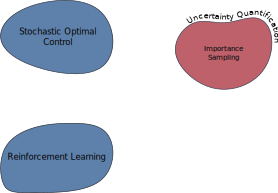
\includegraphics{slides_files/mediabag/img/diagram1.pdf}

\note{What optimization models have we seen in the seminar so far?}
\end{frame}

\begin{frame}
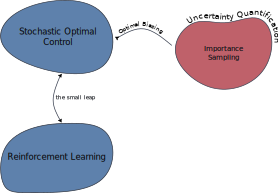
\includegraphics{slides_files/mediabag/img/diagram3.pdf}

\note{\begin{itemize}
\item
  So far we've seen RL as a fancy tool to explore complicated spaces.
  Today, we're going to think of how the discipline of RL as a whole
  introduces new ideas to other areas of mathematics and creates new
  fertile ground.
\item
  Instead of finding ways of computing faster, we're looking for avenues
  to come up with entirely new ways of posing problems that allow us to
  use all of the work that was already invested in ``AI''
\end{itemize}}
\end{frame}

\begin{frame}{Outline}
\phantomsection\label{outline}
\begin{enumerate}
\item
  \emph{Crash} course on RL
\item
  What is importance sampling
\end{enumerate}

\begin{itemize}
\tightlist
\item
  The connection to optimization
\item
  Optimal biasing
\end{itemize}

\begin{enumerate}
\setcounter{enumi}{3}
\tightlist
\item
  Optimal biasing as an RL problem
\end{enumerate}
\end{frame}

\begin{frame}{Crash course on Reinforcement Learning}
\phantomsection\label{crash-course-on-reinforcement-learning}
\pause

\begin{figure}[H]

{\centering 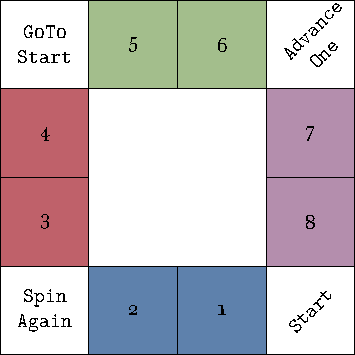
\includegraphics{slides_files/mediabag/img/board.pdf}

}

\caption{A miniopoly board}

\end{figure}%

\note{\begin{itemize}
\tightlist
\item
  I'm training a robot to become the best Miniopoly player
\item
  The rules:

  \begin{itemize}
  \tightlist
  \item
    Players play in turns
  \item
    They move a number of squares determined by a 4-sided dice roll
  \item
    After completing a lap, it gets a reward of \(x\) dollars
  \item
    The trap squares do what it says on the square
  \item
    They can buy property and hotels in the squares.

    \begin{itemize}
    \tightlist
    \item
      If they land of a square someone owns, they pay
    \item
      If someone lands on their square, they charge rent
    \end{itemize}
  \item
    The game ends when someone runs out of money
  \end{itemize}
\end{itemize}}
\end{frame}

\begin{frame}
\begin{itemize}
\tightlist
\item
  The game has a state at turn \(t\) denoted \(s_t\)
\item
  At a turn \(t\) players roll the dice
\item
  The change in money after buying/paying rent/charging rent is recorded
  as a reward \(r_t\)
\end{itemize}

\pause

\begin{tcolorbox}[enhanced jigsaw, coltitle=black, toptitle=1mm, bottomrule=.15mm, leftrule=.75mm, left=2mm, colframe=quarto-callout-important-color-frame, opacityback=0, titlerule=0mm, bottomtitle=1mm, title=\textcolor{quarto-callout-important-color}{\faExclamation}\hspace{0.5em}{Important}, colback=white, toprule=.15mm, breakable, colbacktitle=quarto-callout-important-color!10!white, rightrule=.15mm, opacitybacktitle=0.6, arc=.35mm]

We train our robot to maximize the rewards as it takes actions exploring
the space of states

\end{tcolorbox}

\note{\begin{itemize}
\tightlist
\item
  The state of the game an any given time is information like, who owns
  what squares, how much money they have, in what positions each player
  is, and so on.
\item
  Once a player lands in another square, they can choose to buy it if
  available. If it's not, we carry out the accounting of how much rent
  is, and let the player know how much it won/lost and to what square
  this is connected.
\end{itemize}}

\begin{block}{Can you describe the state space?}
\phantomsection\label{can-you-describe-the-state-space}
\pause

How does it \emph{look} like?
\end{block}

\begin{block}{}
\phantomsection\label{section-1}
It's hard to describe the state space, but we can study the dynamics

\pause

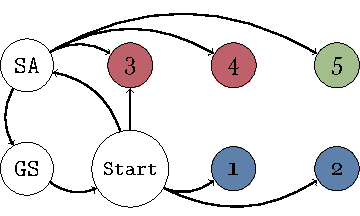
\includegraphics{slides_files/mediabag/img/transicion.pdf}

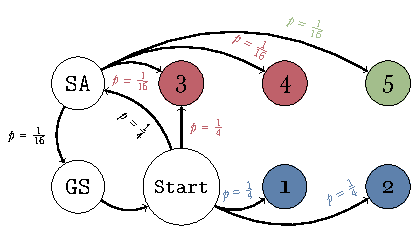
\includegraphics{slides_files/mediabag/img/transicion-markov.pdf}
\end{block}
\end{frame}

\begin{frame}
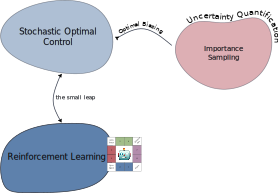
\includegraphics{slides_files/mediabag/img/diagram_rl.pdf}

\note{\begin{itemize}
\tightlist
\item
  We just reviewed very quickly the first bubble
\end{itemize}}

\begin{block}{What if we don't know how square transitions work?}
\phantomsection\label{what-if-we-dont-know-how-square-transitions-work}
\begin{itemize}
\tightlist
\item
  We calculated transition probability \emph{with} the knowledge of the
  dice
\end{itemize}

\pause
\end{block}

\begin{block}{5 minutes to think}
\phantomsection\label{minutes-to-think}
\begin{itemize}
\tightlist
\item
  What is a reasonable way of guessing transition probabilities?
\item
  Can I be sure to observe even improbable but still possible states?
\end{itemize}

The right answers are:

\begin{itemize}
\tightlist
\item
  By simulating the transitions and get empirical estimates
\item
  No
\end{itemize}

\note{\begin{itemize}
\tightlist
\item
  Without knowledge of the dice, we would be left to guess.
\end{itemize}}
\end{block}

\begin{block}{Markov Chain Monte Carlo}
\phantomsection\label{markov-chain-monte-carlo}
\begin{itemize}
\tightlist
\item
  We let the robot roam around and buy squares as it pleases

  \begin{itemize}
  \tightlist
  \item
    For any square, it can either buy it or not
  \end{itemize}
\item
  We register what it gained or lost by buying or not buying a square by
  the end of the game.
\end{itemize}

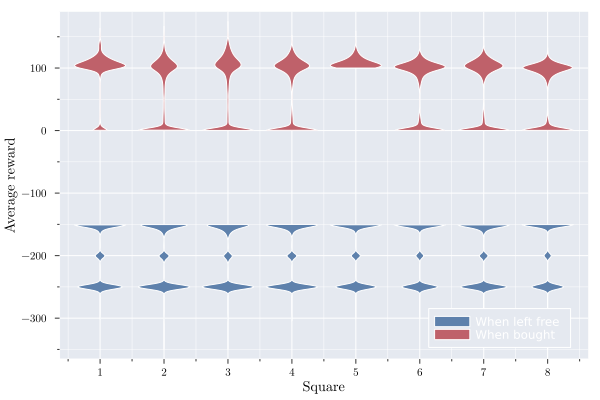
\includegraphics{slides_files/mediabag/img/hist-miniopoly.pdf}

\note{\begin{itemize}
\tightlist
\item
  Graph:

  \begin{itemize}
  \tightlist
  \item
    This is a violin plot. It shows the estimated probability densities
    of observing\ldots{}
  \item
    The x axis shows the different squares
  \item
    The y axis shows the estimated rewards. i.e.~money
  \item
    The red distributions correspond to the expected reward when buying
    a square, while the blue the expected loss when not buying them
  \item
    i.e.~When we buy squares we expect to profit from them, but clearly
    not all squares are as profitable, look at the different shapes of
    the distributions. On the other hand, it looks like losing any given
    square leads to the same expected loss
  \end{itemize}
\end{itemize}}
\end{block}
\end{frame}

\begin{frame}
\begin{figure}[H]

{\centering 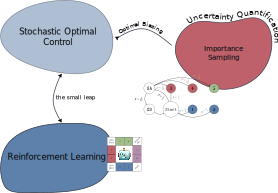
\includegraphics{slides_files/mediabag/img/diagram_IS.pdf}

}

\caption{What we've covered so far}

\end{figure}%

\note{Now we have introduced MCMC as a way for our robot to explore it's
environment and estimate which moves are beneficial to his goal. This is
what the diagram is representing

Moving on\ldots{}}
\end{frame}

\begin{frame}{Importance Sampling}
\phantomsection\label{importance-sampling}
\begin{itemize}
\tightlist
\item
  We wanted to compute the expected reward of the robot after the entire
  game
\item
  Not every problem is this well behaved
\item
  This property is called \emph{metastability}
\item
  Importance sampling aims to remedy this
\end{itemize}

\begin{tcolorbox}[enhanced jigsaw, coltitle=black, toptitle=1mm, bottomrule=.15mm, leftrule=.75mm, left=2mm, colframe=quarto-callout-important-color-frame, opacityback=0, titlerule=0mm, bottomtitle=1mm, title=\textcolor{quarto-callout-important-color}{\faExclamation}\hspace{0.5em}{Important}, colback=white, toprule=.15mm, breakable, colbacktitle=quarto-callout-important-color!10!white, rightrule=.15mm, opacitybacktitle=0.6, arc=.35mm]

The general idea of importance sampling is to draw random variables from
another probability measure and subsequently weight them back in order
to still have an unbiased estimator of the desired quantity of interest

\end{tcolorbox}

\note{\begin{itemize}
\tightlist
\item
  We \textbf{estimated} this quantity by observing and measuring an
  empirical average. But our approximation for extremely unlikely states
  will always be bad by virtue of how little samples we have.
\item
  Many problems, like molecular dynamics, chemical reactions,
  etc\ldots{} have extremely like states, and other extremely unlikely
  states. If we were to use MCMC, we would need impractical amounts of
  time to simulate it and observe every state
\item
  Metastability makes MCMC extremely hard to apply. The variance of our
  estimations is always going to be enormous under these conditions
\item
  We can aim to make sampling faster by reducing the inherent variance
\item
  \textbf{After Callout} In the case of stochastic processes this change
  of measure corresponds to adding a control to the original process
\end{itemize}}
\end{frame}

\begin{frame}
\begin{columns}[T]
\begin{column}{0.48\textwidth}
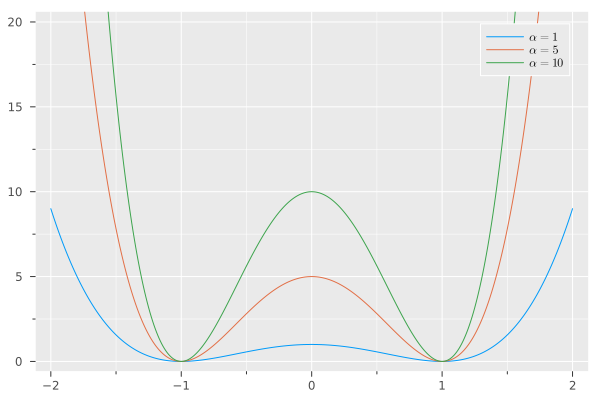
\includegraphics[width=1\textwidth,height=\textheight]{slides_files/mediabag/img/double_well.pdf}
\end{column}

\begin{column}{0.48\textwidth}
\begin{itemize}
\tightlist
\item
  We want to explore space

  \begin{itemize}
  \tightlist
  \item
    We can't make it to the other well
  \end{itemize}
\item
  The jumps are exponentially less probable w.r.t the height of the
  barrier
\end{itemize}
\end{column}
\end{columns}

\note{\begin{itemize}
\tightlist
\item
  It turns out that there is an optimal way to design such a scheme,
  leading to substantially reduced mean hitting times which do not scale
  exponentially with the energy barrier anymore
\end{itemize}}

\begin{block}{More formally\ldots{}}
\phantomsection\label{more-formally}
\begin{itemize}
\tightlist
\item
  The metastable stochastic system we sample from follows Langevin
  dynamics \begin{equation}
  \mathrm{d}X_s = - \nabla V(X_s) \, \mathrm{d}s + \sigma(X_s) \, \mathrm{d}W_s
  \end{equation}
\item
  We want to hit a target set \(\mathcal{T}\). We define
  \begin{equation}
  \tau = \inf \{ s > 0 \mid X_s \in \mathcal{T} \}
  \end{equation}
\item
  We're interested in computing
  \(I: C([0, \infty), \mathbb{R}^d) \to \mathbb{R}\) \begin{equation}
  I(X) \coloneqq \exp(- \mathcal{W}(X))
  \end{equation}
\end{itemize}

\note{\begin{itemize}
\tightlist
\item
  Where:

  \begin{itemize}
  \tightlist
  \item
    \(X_s\) is the position of our particle at time \(s\)
  \item
    \(V\) is a ``potential''
  \item
    We assume there exists a unique strong solution that is ergodic
  \end{itemize}
\item
  Note that \(\tau\) is a.s. finite
\item
  Where \(\mathcal{W}\) serving as a measure of ``work'' over a
  trajectory
\end{itemize}}
\end{block}
\end{frame}

\begin{frame}
Our main goal is to compute \[
  \Psi(X) \coloneqq \mathbb{E}^x [I(X)] \coloneqq \mathbb{E}[I(X) \mid X_0 = x]
\]

But\ldots{}

\pause

\begin{itemize}
\tightlist
\item
  MCMC has terrible properties because of metastability
\item
  No closed form exists
\end{itemize}

\pause

\begin{tcolorbox}[enhanced jigsaw, coltitle=black, toptitle=1mm, bottomrule=.15mm, leftrule=.75mm, left=2mm, colframe=quarto-callout-tip-color-frame, opacityback=0, titlerule=0mm, bottomtitle=1mm, title=\textcolor{quarto-callout-tip-color}{\faLightbulb}\hspace{0.5em}{Tip}, colback=white, toprule=.15mm, breakable, colbacktitle=quarto-callout-tip-color!10!white, rightrule=.15mm, opacitybacktitle=0.6, arc=.35mm]

\begin{itemize}
\tightlist
\item
  We can ``push'' the particle adding force, as long as we account for
  it and correct for that bias
\item
  That ``push'' is achieved by adding a control \(u\).
\end{itemize}

\end{tcolorbox}
\end{frame}

\begin{frame}
The new, controlled dynamics are now described as \begin{equation}
\label{eq: controlled langevin sde}
\mathrm dX_s^u = (-\nabla V(X_s^u) + \sigma(X_s^u)  \,  u(X_s^u))\mathrm ds + \sigma(X_s^u) \mathrm dW_s, \qquad X_0^u = x 
\end{equation}

\pause

Via Girsanov, we can relate our QoI to the original as such:
\begin{equation}
\label{eq: expectation IS}
    \mathbb{E}^x\left[I(X)\right] = \mathbb{E}^x\left[I(X^u) M^u\right],
\end{equation}

\pause

where the exponential martingale \begin{equation}
\label{eq: girsanov martingale}
M^u \coloneqq \exp{\left(-  \int_0^{\tau^u} u(X_s^u) \cdot \mathrm dW_s - \frac{1}{2} \int_0^{\tau^u} |u(X_s^u)|^2 \mathrm ds \right)}
\end{equation} corrects for the bias the pushing introduces.
\end{frame}

\begin{frame}
\begin{tcolorbox}[enhanced jigsaw, coltitle=black, toptitle=1mm, bottomrule=.15mm, leftrule=.75mm, left=2mm, colframe=quarto-callout-important-color-frame, opacityback=0, titlerule=0mm, bottomtitle=1mm, title=\textcolor{quarto-callout-important-color}{\faExclamation}\hspace{0.5em}{Important}, colback=white, toprule=.15mm, breakable, colbacktitle=quarto-callout-important-color!10!white, rightrule=.15mm, opacitybacktitle=0.6, arc=.35mm]

The previous relationship always holds. But the variance of the
estimator depends \emph{heavily} on the choice of \(u\).

\end{tcolorbox}

\pause

Clearly, we aim to achieve the smallest possible variance through on
\emph{optimal control} \(u^*\) \begin{equation}
\label{eq: variance minimization}
\operatorname{Var} \left( I(X^{u^*}) M^{u^*} \right)
= \inf_{u \in \mathcal{U}} \left\{ \operatorname{Var} (I(X^u) M^u) \right\}
\end{equation}

\note{\begin{itemize}
\tightlist
\item
  Where:

  \begin{itemize}
  \tightlist
  \item
    \(X^{u}_{s}\) is the position of our particle at time \(s\) under
    control \(u\)
  \item
    The potential \(u\) is an Itô integrable function satisfying a
    linear growth condition
  \end{itemize}
\item
  Note that \(\tau\) is a.s. finite
\item
  Where \(\mathcal{W}\) serving as a measure of ``work'' over a
  trajectory
\end{itemize}}

\begin{block}{Connection to optimization}
\phantomsection\label{connection-to-optimization}
It turns out \footnote<.->{Feynman--Kac \(\to\) Hopf--Cole
  Transformation \(\to\) Hamilton-Jacobi-Bellman} that the problem of
minimizing variance corresponds to a problem in optimal control

\pause

The cost functional \(J\) to find the variance minimizing control is
\begin{equation}
\label{eq: cost functional}
J(u; x) \coloneqq \mathbb{E}^x\left[\mathcal{W}(X^u) + \frac{1}{2} \int_0^{\tau^u} |u(X_s^u)|^2 \mathrm ds \right],
\end{equation}
\end{block}
\end{frame}

\begin{frame}
With this formulation, \begin{equation}
    \Phi(x) = \inf_{u \in \mathcal{U}} J(u; x).
\end{equation}

\begin{tcolorbox}[enhanced jigsaw, coltitle=black, toptitle=1mm, bottomrule=.15mm, leftrule=.75mm, left=2mm, colframe=quarto-callout-important-color-frame, opacityback=0, titlerule=0mm, bottomtitle=1mm, title=\textcolor{quarto-callout-important-color}{\faExclamation}\hspace{0.5em}{Important}, colback=white, toprule=.15mm, breakable, colbacktitle=quarto-callout-important-color!10!white, rightrule=.15mm, opacitybacktitle=0.6, arc=.35mm]

The optimal bias achieves zero variance: \begin{equation}
    \operatorname{Var} \left( I(X^{u^*}) M^{u^*} \right) = 0.
\end{equation}

\end{tcolorbox}
\end{frame}

\begin{frame}{Optimal biasing through RL}
\phantomsection\label{optimal-biasing-through-rl}
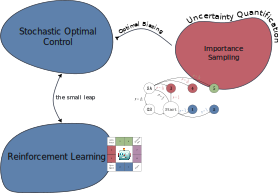
\includegraphics{slides_files/mediabag/img/diagram_complete.pdf}
\end{frame}

\begin{frame}
\begin{itemize}
\tightlist
\item
  Let's reconsider the SOC problem (excuse the change in notation)
\item
  We discretize the dynamics equation \begin{align*}
  s_{t+1} &= s_t + \left( -\nabla V(s_t)  + \sigma u(s_t)\right) \Delta t + \sigma \, \sqrt{\Delta t} \, \eta_{t+1} \\
  s_0 &= x
  \end{align*}
\end{itemize}

\note{\begin{itemize}
\tightlist
\item
  Sorry for the slightly different notation
\item
  Where

  \begin{itemize}
  \tightlist
  \item
    Our state is now represented by \(s\)
  \item
    We have the same potential \(V\)
  \item
    The diffusion term is \(\sigma\) again
  \item
    \(\Delta t\) is the length of the time step
  \item
    The term \(\sqrt{\Delta t} \eta_{t+1}\) is a Brownian increment,
    \(\eta_t \sim N(0, 1)\)
  \end{itemize}
\end{itemize}}
\end{frame}

\begin{frame}
The time-discretized objective function is given by \begin{equation}
\small
J(u; x) \coloneqq \mathbb{E}^{x} \left[ g(s_{T_u}) + \sum_{t=0}^{T_{u-1}} f(s_t) \Delta t + \frac{1}{2} \sum_{t=0}^{T_{u-1}} |u(s_t)|^2 \Delta t \right]
\end{equation}

\begin{itemize}
\tightlist
\item
  Our stopping time \(\tau\) is now denoted \(T_u\)
\end{itemize}
\end{frame}

\begin{frame}
\begin{itemize}
\tightlist
\item
  The return we want to optimize depends on a rewards function \[
  r_t = r(s_t, a_t) \coloneqq
  \begin{cases}
  - f(s_t) \Delta t - \frac{1}{2} |a_t|^2 \Delta t & \text{if} \; s_t \notin \mathcal{T} \\
  -g(s_t) & \text{if} \quad s_t \in \mathcal{T}.
  \end{cases}
  \]
\end{itemize}

\note{\begin{itemize}
\tightlist
\item
  The reward function is defined such that the corresponding return
  along a trajectory equals the negative term inside the expectation of
  the time-discretized cost functional
\item
  Notice that the reward signal is in general not sparse since the agent
  receives feedback at each time step but the choice of the running cost
  f and the final cost g can influence this statement.
\end{itemize}}
\end{frame}

\begin{frame}
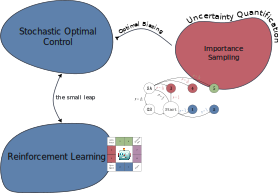
\includegraphics{slides_files/mediabag/img/diagram_complete.pdf}
\end{frame}

\begin{frame}{References}
\phantomsection\label{references}
\phantomsection\label{refs}
\begin{CSLReferences}{1}{0}
\bibitem[\citeproctext]{ref-BorrellConnecting24}
Quer, J., and Enric Ribera Borrell. 2024. {``Connecting Stochastic
Optimal Control and Reinforcement Learning.''} \emph{Journal of
Mathematical Physics} 65. \url{https://doi.org/10.1063/5.0140665}.

\bibitem[\citeproctext]{ref-riberaborrellImprovingControlBased2024}
Ribera Borrell, Enric, Jannes Quer, Lorenz Richter, and Christof
Schütte. 2024. {``Improving {Control Based Importance Sampling
Strategies} for {Metastable Diffusions} via {Adapted Metadynamics}.''}
\emph{SIAM Journal on Scientific Computing} 46 (2): S298--323.
\url{https://doi.org/10.1137/22M1503464}.

\end{CSLReferences}
\end{frame}




\end{document}
